\icsyncex{1}

\begin{exercise}\label{ex:cw-no-pushouts}
设 $h(\mathrm{CW})$ 为 \trCWComplex{}的\trHomotopyCategory{}。证明这个范畴并不拥有
全部\trPushout{}。更具体地，证明图表
\[
\ast \longleftarrow S^1 \xrightarrow{\ \cdot 2\ } S^1
\]
不容许\trPushout{}。
\end{exercise}

\begin{exercise}\label{ex:simplicial-identities}
推导出下列\emph{单纯恒等式}（simplicial identities）中的至少三个：
\begin{enumerate}[label=(\arabic*)]
  \item $d_i^* d_j^* = d_{j-1}^* d_i^*$，若 $i < j$；
  \item $d_i^* s_j^* = s_{j-1}^* d_i^*$，若 $i < j$；
  \item $d_i^* s_j^* = \mathrm{id}$，若 $i = j$ 或 $i = j + 1$；
  \item $d_i^* s_j^* = s_j^* d_{i-1}^*$，若 $i > j + 1$；%
  \footnote{译注：原书此处条件印作「$i > i + 1$」，按恒等式本身应为
  $i > j + 1$，兹改。}
  \item $s_i^* s_j^* = s_{j+1}^* s_i^*$，若 $i \le j$。
\end{enumerate}
这里，对任意\trSimplicialSet{} $X\colon \Delta^{\mathrm{op}} \to \mathrm{Set}$，我们把
映射 $X(d_i)$ 记作 $d_i^*$。提示：想想这条规定对 $\Delta$ 中的映射 $d_i$ 与 $s_j$
意味着什么，并在 $\Delta$ 中先证明相应的恒等式。
\end{exercise}

\begin{exercise}\label{ex:delta-epi-mono-factorization}
证明 $\Delta$ 中的每个映射都可以唯一地分解成若干个 $s_i$ 的复合后接若干个 $d_j$
的复合。因此，一个\trSimplicialSet{}等价地由一列集合 $X_n$ 连同满足单纯恒等式的%
\trFaceMap{}与\trDegeneracyMap{}所描述。
\end{exercise}

\begin{exercise}\label{ex:pi0-relation-not-equivalence}
举出\trSimplicialSet{}的例子，使得第 1 章中的\cref{def:pi0}里导出
$\pi^{\Delta}_0(X)$ 的那个关系既不对称、也不传递。
\end{exercise}

\begin{exercise}\label{ex:eilenberg-zilber}
证明每个\trSimplex{} $x \in X_n$ 都形如 $\alpha^*(y)$，其中 $\alpha\colon [n] \to [m]$
是一个满射，$y$ 是一个\trNonDegenerate{} $m$-\trSimplex{}；并证明对 $(\alpha, y)$ 由 $x$
唯一确定。%
\footnote{译注：原书此处把 $\alpha$ 印作 $\alpha\colon [m] \to [n]$、把 $y$ 印作%
\trNonDegenerate{}%
$n$-\trSimplex{}；按 $\alpha^*$ 的类型规则（$\alpha^*\colon X_m \to X_n$）应为
$\alpha\colon [n] \to [m]$ 与\trNonDegenerate{} $m$-\trSimplex{}，兹改。}
\end{exercise}

\begin{exercise}\label{ex:set-bicomplete}
证明\trCategory{} $\mathrm{Set}$ 是\trBicomplete{}。提示：一般的\trColimit{}可构造为
不交并的商，而一般的\trLimit{}可构造为\trProduct{}的子集。
\end{exercise}

\begin{exercise}\label{ex:colimit-initial-cocone}
设 $F\colon I \to \mathcal{C}$ 是一个\trFunctor{}。证明 $F$ 的\trColimit{}可以等价地
描述为 $F$ 之上的始余锥（initial cocone），而 $F$ 的\trLimit{}可以等价地描述为
$F$ 之上的终锥（terminal cone）。
\end{exercise}

\begin{exercise}\label{ex:limit-colimit-simplicial-set}
计算\trSimplicialSet{} $X\colon \Delta^{\mathrm{op}} \to \mathrm{Set}$ 的\trLimit{}与%
\trColimit{}。
\end{exercise}

\begin{exercise}\label{ex:adjunction-unit-counit}
证明第 1 章中的定义 1.1.17 意义下的一个\trAdjunction{}的数据，等价于
一对\trFunctor{} $(F, G)$ 连同满足三角恒等式（triangle identities）的%
\trNaturalTransformation{} $\varepsilon\colon FG \to \mathrm{id}$ 与
$\eta\colon \mathrm{id} \to GF$，也就是说，显然的复合%
\footnote{译注：原书此处把 $\eta$ 的方向印作「$\eta\colon GF \to \mathrm{id}$」；按其下
所列的两个复合，应为 $\eta\colon \mathrm{id} \to GF$，兹改。}
\[
F(X) \to F(GF(X)) \cong FG(FX) \to F(X)
\]
与
\[
G(X) \to GF(G(X)) \cong G(FG(X)) \to G(X)
\]
分别是 $F(X)$ 与 $G(X)$ 的恒等映射。
\end{exercise}

\begin{exercise}\label{ex:adjoint-via-hom-bijection}
设 $F\colon \mathcal{C} \to \mathcal{D}$ 是一个\trFunctor{}。如果你能为所有
$y \in \mathcal{D}$ 指定\trObject{} $Gy$ 与映射 $\varepsilon_y\colon FGy \to y$，使得
态射集上的诱导映射
\[
\mathrm{Hom}_{\mathcal{C}}(x, Gy)
\xrightarrow{\ F\ }
\mathrm{Hom}_{\mathcal{D}}(Fx, FGy)
\xrightarrow{\ \varepsilon_y\ }
\mathrm{Hom}_{\mathcal{D}}(Fx, y)
\]
是双射，那么 $F$ 容许一个\trRightAdjoint{}。注意，有一个显然的对偶概念，它表明：
若能为所有 $y \in \mathcal{D}$ 指定\trObject{} $Gy$ 与映射 $\eta_y\colon y \to FGy$，
使得态射集上的诱导映射
\[
\mathrm{Hom}_{\mathcal{D}}(Gy, x)
\xrightarrow{\ F\ }
\mathrm{Hom}_{\mathcal{C}}(FGy, Fx)
\xrightarrow{\ \eta_y\ }
\mathrm{Hom}_{\mathcal{C}}(y, Fx)
\]
是双射，那么 $F$ 容许一个\trLeftAdjoint{}。
\end{exercise}

\begin{exercise}\label{ex:product-nondegenerate-dimension}
证明：若\trSimplicialSet{} $X$ 至多拥有 $n$ 维的\trNonDegenerate{}\trSimplex{}，$Y$
至多拥有 $m$ 维的\trNonDegenerate{}\trSimplex{}，则它们的乘积 $X \times Y$ 至多拥有
$(n + m)$ 维的\trNonDegenerate{}\trSimplex{}。
\end{exercise}

\begin{exercise}\label{ex:pi0-realization}
证明：对每个\trSimplicialSet{} $X$，存在典范双射
$\pi^{\Delta}_0(X) \cong \pi_0(|X|)$。
\end{exercise}

\begin{exercise}\label{ex:spine-horn-boundary-inclusions}
证明：当 $0 < j < n$ 或 $n \ge 3$ 时，有包含 $I^n \subseteq \Lambda^n_j$；并且对%
所有 $n \ge 0$，有 $\Lambda^n_j \subseteq \partial\Delta^n \subseteq \Delta^n$。
\end{exercise}

\begin{exercise}\label{ex:limit-initial-object}
设 $I$ 是一个拥有\trInitialObject{} $i$ 的\trCategory{}，$J$ 是一个拥有%
\trTerminalObject{} $t$ 的\trCategory{}。证明：\trFunctor{} $F\colon I \to \mathcal{C}$
的一个\trLimit{}由 $F(i)$（连同对所有 $x \in I$ 的典范映射
$F(i) \to F(x)$）给出。类似地，证明\trFunctor{} $G\colon J \to \mathcal{C}$ 的一个%
\trColimit{}由 $G(t)$（连同其对所有 $x \in J$ 的映射 $G(x) \to G(t)$）给出。
\end{exercise}

\begin{exercise}\label{ex:skeleton-pushout-filtration}
证明：对每个 $n \ge 0$，有\trPushout{}%
\begin{center}
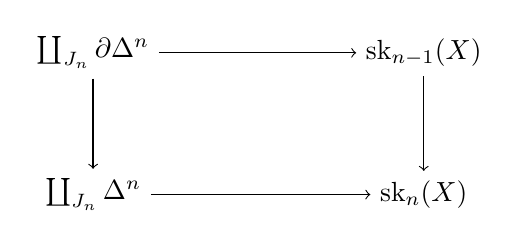
\begin{tikzpicture}
  \node (a) at (0,0) {$\coprod_{J_n} \partial\Delta^n$};
  \node (b) at (4.2,0) {$\mathrm{sk}_{n-1}(X)$};
  \node (c) at (0,-1.8) {$\coprod_{J_n} \Delta^n$};
  \node (d) at (4.2,-1.8) {$\mathrm{sk}_n(X)$};
  \draw[->] (a) -- (b);
  \draw[->] (a) -- (c);
  \draw[->] (b) -- (d);
  \draw[->] (c) -- (d);
\end{tikzpicture}
\end{center}
其中 $J_n$ 是\trNonDegenerate{} $n$-\trSimplex{}之集。此外，证明
$X \cong \mathrm{colim}_n\,\mathrm{sk}_n(X)$。
\end{exercise}

\begin{exercise}\label{ex:not-nerves-of-categories}
证明下列单纯集都不是\trCategory{}的\trNerve{}：
\begin{enumerate}[label=(\arabic*)]
  \item $n \ge 2$ 时的 $\partial\Delta^n$；
  \item $n \ge 2$ 且 $0 \le j \le n$ 时的 $\Lambda^n_j$；
  \item $n \ge 2$ 时的 $I^n$。
\end{enumerate}
\end{exercise}

\begin{exercise}\label{ex:coskeleton-kan}
设 $X$ 是一个 \trKanComplex{}。证明：对所有 $n \ge 0$，\trSimplicialSet{}%
$\mathrm{cosk}_n(X)$ 仍是一个 \trKanComplex{}。证明典范映射
$X \to \mathrm{cosk}_n(X)$ 诱导双射
\[
\pi^{\Delta}_k(X) \to \pi^{\Delta}_k(\mathrm{cosk}_n(X))
\]
（当 $k < n$），并且 $\pi^{\Delta}_k(\mathrm{cosk}_n(X)) = 0$（当 $k \ge n$）。
\end{exercise}

\begin{exercise}\label{ex:natural-transformation-homotopy}
证明：\trFunctor{} $f, g\colon \mathcal{C} \to \mathcal{D}$ 之间的一个%
\trNaturalTransformation{}诱导 $\mathrm{N}(f)$ 与
$\mathrm{N}(g)\colon \mathrm{N}(\mathcal{C}) \to \mathrm{N}(\mathcal{D})$ 之间的一个%
\trHomotopy{}。利用这个结果证明：用一个元素作共轭，确定了分类空间 $BG$ 的一个
同伦于恒等的自映射。这个共轭在 $\pi_1(BG)$ 上诱导了什么？为什么这并不表明每个群
都是交换的？
\end{exercise}

\begin{exercise}\label{ex:nerve-2-coskeletal}
证明\trCategory{} $\mathcal{C}$ 的\trNerve{}是 $2$-\trCoskeleton{}的，也就是说，
典范映射 $\mathrm{N}(\mathcal{C}) \to \mathrm{cosk}_2(\mathrm{N}(\mathcal{C}))$ 是%
\trSimplicialSet{}的同构。
\end{exercise}

\begin{exercise}\label{ex:skeleton-coskeleton-idempotent}
设 $X$ 是一个\trSimplicialSet{}，$n \le m$。证明
$\mathrm{sk}_n(\mathrm{sk}_m(X)) = \mathrm{sk}_n(X) = \mathrm{sk}_m(\mathrm{sk}_n(X))$。
由此推出 $\mathrm{cosk}_n(\mathrm{cosk}_m(X)) \cong \mathrm{cosk}_m(\mathrm{cosk}_n(X))$。
$\mathrm{sk}_n(\mathrm{cosk}_m(X)) \cong \mathrm{cosk}_m(\mathrm{sk}_n(X))$ 也成立吗？
（若不成立：给出一个反例。）这两个单纯集之间有没有一个典范的偏爱映射？
\end{exercise}

\begin{exercise}\label{ex:nerve-op}
设 $\mathcal{C}$ 是一个\trCategory{}，$X$ 是一个\trSimplicialSet{}。回顾：
$X^{\mathrm{op}}$ 是如下定义的\trSimplicialSet{}：$X^{\mathrm{op}}_n = X_n$，而
$d^{\mathrm{op}}_i\colon X_n \to X_{n-1}$ 由 $d_{n-i}$ 给出，同样地 $s^{\mathrm{op}}_i = s_{n-i}$
（作为映射 $X_n \to X_{n+1}$）。证明下述诸断言：
\begin{enumerate}[label=(\arabic*)]
  \item $\mathrm{N}(\mathcal{C}^{\mathrm{op}}) \cong \mathrm{N}(\mathcal{C})^{\mathrm{op}}$
  \item $(\Delta^n)^{\mathrm{op}} \cong \Delta^n$
  \item $(\Lambda^n_i)^{\mathrm{op}} \cong \Lambda^n_{n-i}$
  \item $(\partial\Delta^n)^{\mathrm{op}} \cong \partial\Delta^n$
\end{enumerate}
\end{exercise}

\begin{exercise}\label{ex:bg-homotopy-groups}
设 $G$ 是一个群，$\mathbb{B}G$ 是只有一个\trObject{}、以 $G$ 作为该\trObject{}的
自同态的\trCategory{}。证明 $\mathrm{N}(\mathbb{B}(G))$ 只有一个非平凡的同伦群，即
$\pi^{\Delta}_1(\mathrm{N}(\mathbb{B}G))$，并且这个群典范地同构于 $G$。
\end{exercise}

\begin{exercise}\label{ex:composer-identity-composition}
设 $X$ 是一个\trComposer{}，$f\colon x \to y$ 是 $X$ 中的一个\trMorphism{}。证明 $f$
是 $\mathrm{id}_x$ 与 $f$ 的合成，也是 $f$ 与 $\mathrm{id}_y$ 的合成。
\end{exercise}

\begin{exercise}\label{ex:boundary-not-kan}
考虑 $\Delta$ 中像为 $\{0\}$ 的映射 $[0] \to [n]$。证明这确定了一个映射
$0\colon \Delta^0 \to \partial\Delta^n$。计算单纯同伦集 $\pi^{\Delta}_i(\partial\Delta^n, 0)$
（对 $i \ge 1$ 与 $n \ge 2$）。由此推出 $\partial\Delta^n$ 不是 \trKanComplex{}。
\end{exercise}

\begin{exercise}\label{ex:not-infinity-categories}
证明下列单纯集都不是∞-\trCategories{}：
\begin{enumerate}[label=(\arabic*)]
  \item $n \ge 2$ 时的 $\partial\Delta^n$；
  \item $n \ge 3$ 且 $0 \le j \le n$ 时的 $\Lambda^n_j$；
  \item $n \ge 2$ 时的 $I^n$。
\end{enumerate}
\end{exercise}

\begin{exercise}\label{ex:homotopy-categories-of-standard-examples}
确定下列单纯集的同伦范畴：
\begin{enumerate}[label=(\arabic*)]
  \item $n \ge 1$ 时的 $\partial\Delta^n$；
  \item $n \ge 2$ 且 $0 \le j \le n$ 时的 $\Lambda^n_j$；
  \item $n \ge 0$ 时的 $I^n$。
\end{enumerate}
\end{exercise}

\begin{exercise}\label{ex:homotopy-category-functoriality-failures}
设 $f\colon X \to Y$ 是\trSimplicialSet{}的映射。对下述诸陈述给出证明或反例：
\begin{enumerate}[label=(\arabic*)]
  \item 若 $f$ 是\trMonomorphism{}，则 $hX \to hY$ 是\trFullyFaithful{}；
  \item 若 $f$ 是逐层满射，则 $hX \to hY$ 是\emph{满且全的}（surjective and full），
        也就是说，它在\trObject{}上与在态射集上都诱导满射；
  \item 若 $f$ 在 $0$-\trSimplex{}与 $1$-\trSimplex{}上诱导满射，则
        $hX \to hY$ 满且全。
\end{enumerate}
\end{exercise}

\begin{exercise}\label{ex:h-not-monoidal}
证明或否证下述陈述：对任意两个\trSimplicialSet{} $X$ 与 $Y$，典范映射
$h(X \times Y) \to hX \times hY$ 是\trCategory{}的同构。
\end{exercise}

\begin{exercise}\label{ex:connected-groupoids}
称一个\trCategory{} $\mathcal{C}$ 为\trConnected{}的，若
$\pi^{\Delta}_0(\mathrm{N}(\mathcal{C}))$ 只由一个元素组成。证明：\trGroupoid{}%
$\mathcal{G}$ 是\trConnected{}的，当且仅当对任意两个\trObject{} $x, y \in \mathcal{G}$，集合
$\mathrm{Hom}_{\mathcal{G}}(x, y)$ 非空。证明：\trConnected{}的\trGroupoid{}等价于某个群 $G$
的 $\mathbb{B}G$。然而要证明：由\trConnected{}\trGroupoid{}构成的\trCategory{}\emph{不}等价于
由群构成的\trCategory{}。
\end{exercise}

\begin{exercise}\label{ex:h-singular-category}
设 $X$ 是一个\trTopologicalSpace{}。描述\trCategory{} $h(\mathcal{S}(X))$。证明每个%
\trObject{}的自同态构成一个群。这是哪个群？
\end{exercise}

\begin{exercise}\label{ex:homotopic-square-composer}
设 $X$ 是一个具有内 $3$-角扩张性质的\trComposer{}。设
$\sigma\colon \Delta^1 \times \Delta^1 \to X$ 是一个映射，使得
\begin{enumerate}[label=(\arabic*)]
  \item $\sigma|_{\Delta^1 \times \{0\}} = f$，
  \item $\sigma|_{\Delta^1 \times \{1\}} = g$，
  \item $\sigma|_{\{0\} \times \Delta^1} = \mathrm{id}_x$，并且
  \item $\sigma|_{\{1\} \times \Delta^1} = \mathrm{id}_y$，
\end{enumerate}
其中 $f, g\colon x \to y$ 为\trMorphism{}。证明：在第 1 章中的%
\cref{def:equivalent-1-simplices}的意义下 $f \sim g$。
\end{exercise}

\begin{exercise}\label{ex:composition-space-connected}
设 $X$ 是一个具有内 $3$-角扩张性质的\trComposer{}。证明：对任意两个可合成的%
\trMorphism{} $f\colon x \to y$ 与 $g\colon y \to z$，\trSimplicialSet{}%
$\mathrm{Comp}_X(f, g)$ 是\trConnected{}的，也就是说，
$\pi^{\Delta}_0(\mathrm{Comp}_X(f, g))$ 只由一个元素组成。
\end{exercise}

\begin{exercise}\label{ex:cosk2-vs-nerve-hx}
设 $X$ 是一个\trSimplicialSet{}，考虑典范映射 $X \to \mathrm{N}(hX)$。
\begin{enumerate}[label=(\arabic*)]
  \item 证明该映射穿过典范映射 $X \to \mathrm{cosk}_2(X)$。
  \item 证明：若 $X$ 同构于某个\trCategory{}的\trNerve{}，则诱导映射
        $\mathrm{cosk}_2(X) \to \mathrm{N}(hX)$ 是同构。
  \item 证明映射 $\mathrm{cosk}_2(X) \to \mathrm{N}(hX)$ 一般不是同构。提示：找一个
        $2$-\trCoskeleton{}的、但并非\trCategory{}之\trNerve{}的 $X$。
  \item 证明或否证下述陈述：映射 $\mathrm{cosk}_2(X) \to \mathrm{N}(hX)$ 是同构，
        当且仅当 $X$ 同构于某个\trCategory{}的\trNerve{}。
\end{enumerate}
\end{exercise}

\begin{exercise}\label{ex:hom-v-lax-monoidal}
设 $(V, \otimes, \mathbf{1})$ 是一个幺半范畴。那么\trFunctor{}%
$\mathrm{Hom}_V(\mathbf{1}, -)\colon V \to \mathrm{Set}$ 是一个%
\trLaxMonoidalFunctor{}。它是幺半的吗？若不是：你能在 $(V, \otimes, \mathbf{1})$
上找到一个确保它是幺半的条件吗？
\end{exercise}

\begin{exercise}\label{ex:pointed-lax-monoidal}
设 $\mathcal{C}$ 是一个具有有限\trProduct{}与有限\trCoproduct{}的\trCategory{}。我们称
$\mathcal{C}$ 为\emph{\trPointed{}}（pointed），如果从\trInitialObject{}到%
\trTerminalObject{}的典范映射 $\varnothing \to \ast$ 是同构。证明恒等\trFunctor{}%
典范地精化（refine）为一个\trLaxMonoidalFunctor{}%
$(\mathcal{C}, \times, \ast) \to (\mathcal{C}, \amalg, \varnothing)$。这个\trFunctor{}%
何时是幺半的？此外，证明任意\trFunctor{} $F\colon \mathcal{C} \to \mathcal{D}$ 都
典范地精化为一个对称松幺半\trFunctor{}%
$(\mathcal{C}, \amalg, \varnothing) \to (\mathcal{D}, \amalg, \varnothing)$。
它何时是幺半的？
\end{exercise}

\begin{exercise}\label{ex:essentially-surjective-fully-faithful-equivalence}
本练习的目标是证明：通常\trCategories{}之间任何\trEssentiallySurjective{}且%
\trFullyFaithful{}\trFunctor{} $F\colon \mathcal{C} \to \mathcal{D}$ 都是一个%
\trEquivalence{}。
\begin{enumerate}[label=(\arabic*)]
  \item 证明 $F$ 容许一个伴随 $G$。提示：利用\cref{ex:adjoint-via-hom-bijection}。
  \item 证明 $G$ 本身是\trFullyFaithful{}。
  \item 证明：由\trFullyFaithful{}\trFunctor{}组成的伴随对 $(F, G)$ 使 $F$ 成为一个%
        \trEquivalence{}，且 $G$ 是其逆。
\end{enumerate}
\end{exercise}

\begin{exercise}\label{ex:mutually-inverse-conservative}
设 $F\colon \mathcal{C} \to \mathcal{D}$ 是一个带有\trRightAdjoint{}%
$G\colon \mathcal{D} \to \mathcal{C}$ 的\trFunctor{}。证明：若 $F$ 是\trFullyFaithful{}且
$G$ 是\trConservative{}，则二者互逆。这里，保守性意为：若 $f\colon x \to y$ 是
$\mathcal{D}$ 中的一个\trMorphism{}而 $G(f)$ 是同构，则 $f$ 是同构。
\end{exercise}

\begin{exercise}\label{ex:oplax-lax-transfer}
设 $F\colon \mathcal{C} \to \mathcal{D}$ 左伴随于 $G\colon \mathcal{D} \to \mathcal{C}$。
证明：若 $G$ 是松幺半的，则 $F$ 典范地精化为一个\trOplaxMonoidalFunctor{}。反之，证明：
若 $F$ 是反松幺半的，则 $G$ 典范地精化为一个\trLaxMonoidalFunctor{}。
\end{exercise}

\begin{exercise}\label{ex:monoidal-adjunction-left-adjoint-monoidal}
证明：\trMonoidalAdjunction{}的\trLeftAdjoint{}事实上是幺半的。回顾：一个%
\trMonoidalAdjunction{}由松幺半\trFunctor{} $F$ 与 $G$ 组成，它们由一个单位 $\eta$
与一个余单位 $\varepsilon$ 见证为伴随，其中 $\eta$ 与 $\varepsilon$ 都是幺半变换。
\end{exercise}

\begin{exercise}\label{ex:monoidal-f-adjunction}
设 $F$ 左伴随于 $G$，并由单位与余单位 $(\eta, \varepsilon)$ 所见证。证明：若 $F$
是幺半的，则\cref{ex:oplax-lax-transfer}在 $G$ 上诱导的\trLaxMonoidalFunctor{}结构使
$(F, G, \eta, \varepsilon)$ 成为一个\trMonoidalAdjunction{}。
\end{exercise}

\begin{exercise}\label{ex:coherent-nerve-coproducts}
证明\trCoherentNerve{}\trFunctor{}%
$\mathrm{N}\colon \mathrm{Cat}_{\Delta} \to \mathrm{sSet}$ 与\trCoproduct{}交换。证明
$c$ 不是 $\mathrm{N}$ 的\trRightAdjoint{}。$\mathrm{N}$ 究竟有没有\trRightAdjoint{}？
提示：通常的\trNerve{}\trFunctor{} $\mathrm{N}\colon \mathrm{Cat} \to \mathrm{sSet}$
有没有\trRightAdjoint{}？这两个问题有何关联？
\end{exercise}

\begin{exercise}\label{ex:coherent-nerve-bsimp}
证明：若一个单纯\trCategory{}的\trCoherentNerve{} $\mathrm{N}(\mathcal{C})$ 同构于某个
通常\trCategory{}的\trNerve{}，则底\trCategory{} $u\mathcal{C}$ 同构于\trHomotopyCategory{}%
$\pi(\mathcal{C})$。显式地写出下述单纯\trCategory{}%
$\mathbb{B}^{\mathrm{simp}}(G)$ 的\trCoherentNerve{}：它只有一个\trObject{}，且该%
\trObject{}的自同态单纯集由 $\mathrm{N}(G)$ 给出，其中 $G$ 是一个群（如果你愿意，
也可以是幺半群）。由显式分析推出：$\mathrm{N}(\mathbb{B}^{\mathrm{simp}}(G))$ 不同构于
任何\trCategory{}的\trNerve{}，尽管 $u\mathrm{N}(\mathbb{B}^{\mathrm{simp}}(G)) \cong \pi(\mathrm{N}(\mathbb{B}^{\mathrm{simp}}(G)))$。
\end{exercise}

\begin{exercise}\label{ex:coherent-nerve-existence}
证明或否证下述诸陈述：
\begin{enumerate}[label=(\arabic*)]
  \item 存在一个单纯\trCategory{} $\mathcal{C}$，其\trCoherentNerve{}%
        $\mathrm{N}(\mathcal{C})$ 不是∞-\trCategory{}。
  \item 存在一个单纯\trCategory{} $\mathcal{C}$，其\trCoherentNerve{}%
        $\mathrm{N}(\mathcal{C})$ 是∞-\trCategory{}，但不是 \trKanComplex{}。
\end{enumerate}
\end{exercise}

\begin{exercise}\label{ex:simplicial-equivalence-weakly-fully-faithful}
设 $\mathcal{C}$ 是一个诸态射单纯集全是 \trKanComplex{} 的单纯\trCategory{}。具体地
算出：单纯\trCategory{}中的一个\trMorphism{} $f\colon x \to y$ 是一个\trEquivalence{}%
意味着什么。借助这个结果，重新表述\trWeaklyFullyFaithful{}\trFunctor{}的条件。
\end{exercise}

\begin{exercise}\label{ex:mono-not-subcategory}
证明：存在\trMonomorphism{} $X \to Y$，使得 $X$ 与 $Y$ 都是∞-\trCategories{}，但 $X$
并不是第 1 章中的\cref{def:sub-infinity-category}意义下的子∞-\trCategory{}。
\end{exercise}

\begin{exercise}\label{ex:singular-subcategory}
设 $Y \to X$ 是\trTopologicalSpace{}的一个包含。诱导映射 $\mathcal{S}(Y) \to \mathcal{S}(X)$
何时是一个子\trCategory{}？何时是一个满子\trCategory{}？
\end{exercise}

\begin{exercise}\label{ex:functor-category-full-sub}
设 $\mathcal{C}_0 \subseteq \mathcal{C}$ 是一个满子∞-\trCategory{}，$\mathcal{D}$ 是一个
∞-\trCategory{}。证明\trFunctor{}范畴 $\mathrm{Fun}(\mathcal{D}, \mathcal{C}_0)$ 是
$\mathrm{Fun}(\mathcal{D}, \mathcal{C})$ 的、由那些穿过包含
$\mathcal{C}_0 \subseteq \mathcal{C}$ 的\trFunctor{} $f\colon \mathcal{D} \to \mathcal{C}$
组成的满子∞-\trCategory{}。
\end{exercise}

\begin{exercise}\label{ex:op-infinity-category}
证明：\trSimplicialSet{} $X$ 是∞-\trCategory{}，当且仅当 $X^{\mathrm{op}}$ 是%
∞-\trCategory{}；同样地，$X$ 是 \trKanComplex{}，当且仅当 $X^{\mathrm{op}}$ 是%
\trKanComplex{}。再证明：若 $X$ 是∞-\trCategory{}，则 $X$ 是\trInfinityGroupoid{}%
当且仅当 $X^{\mathrm{op}}$ 是\trInfinityGroupoid{}。
\end{exercise}

\begin{exercise}\label{ex:coherent-nerve-image-of-c}
设 $\mathcal{C}$ 是一个单纯\trCategory{}。证明：\trCoherentNerve{}%
$\mathrm{N}(\mathcal{C})$ 同构于某个通常\trCategory{}的\trNerve{}，当且仅当
$\mathcal{C}$ 落在\trFunctor{} $c\colon \mathrm{Cat} \to \mathrm{Cat}_{\Delta}$ 的像之中。
\end{exercise}

\begin{exercise}\label{ex:h-n-pi}
证明复合
\[
\mathrm{Cat}_{\Delta}
\xrightarrow{\ \mathrm{N}\ }
\mathrm{sSet}
\xrightarrow{\ h\ }
\mathrm{Cat}
\]
同构于\trFunctor{} $\pi\colon \mathrm{Cat}_{\Delta} \to \mathrm{Cat}$。
\end{exercise}

\begin{exercise}\label{ex:inner-fibration-op}
证明下述诸断言：
\begin{enumerate}[label=(\arabic*)]
  \item 设 $\mathcal{C}$ 是一个通常\trCategory{}，$X$ 是一个\trSimplicialSet{}。那么
        $X$ 是∞-\trCategory{}，当且仅当每个映射 $X \to \mathrm{N}(\mathcal{C})$ 都是
        一个\trInnerFibration{}。
  \item 映射 $f\colon X \to Y$ 是\trInnerFibration{}，当且仅当
        $f^{\mathrm{op}}\colon X^{\mathrm{op}} \to Y^{\mathrm{op}}$ 是%
        \trInnerFibration{}。
  \item 映射 $f\colon X \to Y$ 是\trLeftFibration{}，当且仅当映射
        $f^{\mathrm{op}}\colon X^{\mathrm{op}} \to Y^{\mathrm{op}}$ 是%
        \trRightFibration{}。
\end{enumerate}
\end{exercise}

\begin{exercise}\label{ex:chi-galois}
设 $S \subseteq S'$ 是由\trMorphism{}组成的集合。证明：在第 1 章中的\cref{def:chi}
的记号下，
\begin{enumerate}[label=(\arabic*)]
  \item $\chi_R(S') \subseteq \chi_R(S)$；
  \item $S \subseteq \chi(S)$；
  \item $\chi_R(S) = \chi_R(\chi(S))$。
\end{enumerate}
\end{exercise}

\begin{exercise}\label{ex:filtered-poset-characterization}
称一个\trCategory{} $I$ 为\emph{\trFiltered{}}，若从有限\trCategory{} $K$ 出发的每个%
\trFunctor{} $K \to I$ 都能沿包含 $K \to K^{\rhd}$ 延拓。证明：偏序集（视为一个%
\trCategory{}）是\trFiltered{}，当且仅当
\begin{enumerate}[label=(\arabic*)]
  \item 对 $I$ 中对象的每个有限族 $X_1, \dots, X_n$，存在 $I$ 的一个\trObject{} $X$
        连同对所有 $k = 1, \dots, n$ 的映射 $X_k \to X$；
  \item 任意两个\trMorphism{} $f, g\colon X \to Y$ 都可被等化，也就是说，存在一个%
        \trMorphism{} $h\colon Y \to Z$ 使得 $hf = hg$。
\end{enumerate}
\end{exercise}

\begin{exercise}\label{ex:finite-filtered-categories}
设 $I$ 是一个有限\trCategory{}。
\begin{enumerate}[label=(\arabic*)]
  \item 证明：若 $I$ 拥有一个\trTerminalObject{}，则 $I$ 是\trFiltered{}。
  \item 证明：存在 $I$ 是\trFiltered{}但没有\trTerminalObject{}的例子。
  \item 证明：$I$ 是偏序集且是\trFiltered{}，当且仅当它拥有一个%
        \trTerminalObject{}。
\end{enumerate}
特别地，请注意这表明存在大量并非偏序集的\trFiltered{}范畴。
\end{exercise}

\begin{exercise}\label{ex:finitely-presented-compact}
证明：每个只拥有有限多个\trNonDegenerate{}\trSimplex{}的\trSimplicialSet{} $A$
都是\emph{\trCompact{}}，也就是说，只要 $I$ 是\trFiltered{}范畴，典范映射
\[
\mathop{\mathrm{colim}}_{i \in I}\,
\mathrm{Hom}_{\mathrm{sSet}}(A, X_i)
\to
\mathrm{Hom}_{\mathrm{sSet}}\Bigl(A, \mathop{\mathrm{colim}}_{i \in I} X_i\Bigr)
\]
就是同构。
\end{exercise}

\begin{exercise}\label{ex:semi-saturated}
我们称一个映射之集 $S$ 为\emph{半饱和的}（semi-saturated），如果它对推出、%
\trRetract{}与
可数合成封闭。证明半饱和集
\begin{enumerate}[label=(\arabic*)]
  \item 包含全部同构，并且对有限\trCoproduct{}封闭，只要它包含某个\trInitialObject{}%
        $\varnothing$ 的恒等；
  \item 对合成封闭，也就是说，若 $f\colon A \to B$ 与 $g\colon B \to C$ 是 $S$
        的元素，则 $gf\colon A \to C$ 也是；
  \item 若对有限\trCoproduct{}封闭，则对可数\trCoproduct{}封闭，也就是说，若
        $\{f_i\colon A_i \to B_i\}_{i \in I}$ 是 $S$ 中元素的可数族，则映射
        $\coprod_{i \in I} f_i\colon \coprod_{i \in I} A_i \to \coprod_{i \in I} B_i$%
        \footnote{译注：原书此处漏印 $\coprod$ 之作用对象，依上下文补足。——译者注}
        也是 $S$ 中的元素。
\end{enumerate}
\end{exercise}

\begin{exercise}\label{ex:saturated-contains-isos}
证明：\trCategory{} $\mathcal{C}$ 中的\trSaturatedSet{} $S$ 包含全部同构。找一个\trCategory{}%
$\mathcal{C}$ 与 $\mathcal{C}$ 中一个非空、但并不包含全部同构的半饱和\trMorphism{}集
$S$ 的例子。
\end{exercise}

\begin{exercise}\label{ex:generating-maps-set}
证明下述诸断言：
\begin{enumerate}[label=(\arabic*)]
  \item $\mathrm{Set}$ 中的映射 $\varnothing \to \{\ast\}$ 生成单射之集。
        $\chi_R(\varnothing \to \ast)$ 是什么？请显式写出小对象论证对集合的一般映射
        $f\colon M \to N$ 所给出的分解。
  \item 映射 $\{\ast, \ast\} \to \{\ast\}$ 生成满射这一类。
        $\chi_R(\{\ast, \ast\} \to \ast)$ 是什么？请显式写出小对象论证对集合的一般映射
        $f\colon M \to N$ 所给出的分解。
\end{enumerate}
\end{exercise}

\begin{exercise}\label{ex:chi-boundary-inclusions}
考虑由\trBoundaryInclusion{}给出的集合
$S = \{\partial\Delta^n \to \Delta^n\}_{n \ge 0}$。证明 $\chi(S)$ 恰由\trSimplicialSet{}%
的全部\trMonomorphism{}给出。
\end{exercise}

\begin{exercise}\label{ex:J-not-compact}
证明 $J$ 不是\trCompact{}\trSimplicialSet{}，也就是说，$J$ 中有无穷多个%
\trNonDegenerate{}%
\trSimplex{}。
\end{exercise}

\begin{exercise}\label{ex:extension-over-J-equivalence}
证明：若∞-\trCategory{}中的一个\trMorphism{} $f\colon \Delta^1 \to \mathcal{C}$ 能沿
包含 $\Delta^1 \to J$ 延拓，则 $f$ 是一个\trEquivalence{}。
\end{exercise}

\begin{exercise}\label{ex:horn-retract-pushout-product}
补全第 1 章中的\cref{lem:left-box-generators}的缺失步骤。更精确地，证明下述诸断言：
\begin{enumerate}[label=(\arabic*)]
  \item 对 $0 \le j < n$，\trHornInclusion{} $\Lambda^n_j \to \Delta^n$ 是推出积映射
        \[
        \Delta^n \times \{0\} \amalg_{\Lambda^n_j \times \{0\}} \Lambda^n_j \times \Delta^1
        \to \Delta^n \times \Delta^1
        \]
        的一个\trRetract{}；
  \item 推出积映射
        \[
        \partial\Delta^n \times \Delta^1 \cup \Delta^n \times \{0\}
        \to \Delta^n \times \Delta^1
        \]
        是\trLeftAnodyne{}的。
\end{enumerate}
\end{exercise}

\begin{exercise}\label{ex:trivial-fibration-pi-kan}
证明：\trKanComplex{}之间的\trTrivialFibration{} $f\colon X \to Y$ 在\trCategory{}%
$\pi(\mathrm{Kan})$ 中诱导一个同构。提示：证明 \trKanComplex{}之间的%
\trTrivialFibration{}是一个\trHomotopyEquivalence{}。
\end{exercise}

\begin{exercise}\label{ex:composition-homotopy-equivalence}
证明：若 $f\colon y \to z$ 是一个\trEquivalence{}，则
\[
\mathrm{map}_{\mathcal{C}}(x, y) \simeq
\mathrm{map}_{\mathcal{C}}(x, y) \times \Delta^0
\xrightarrow{\ f\ }
\mathrm{map}_{\mathcal{C}}(x, y) \times \mathrm{map}_{\mathcal{C}}(y, z)
\to
\mathrm{map}_{\mathcal{C}}(x, z)
\]
是一个\trHomotopyEquivalence{}。
\end{exercise}

\begin{exercise}\label{ex:composition-enriched-hkan}
证明：紧接第 1 章中的\cref{def:mapping-infinity-category}之前定义的合成在同伦意义下
结合，也就是说，∞-\trCategory{}中的合成确定了一个充实于 $h(\mathrm{Kan})$（即%
\trKanComplex{}的\trHomotopyCategory{}）的\trCategory{}。提示：考虑图表
\begin{center}
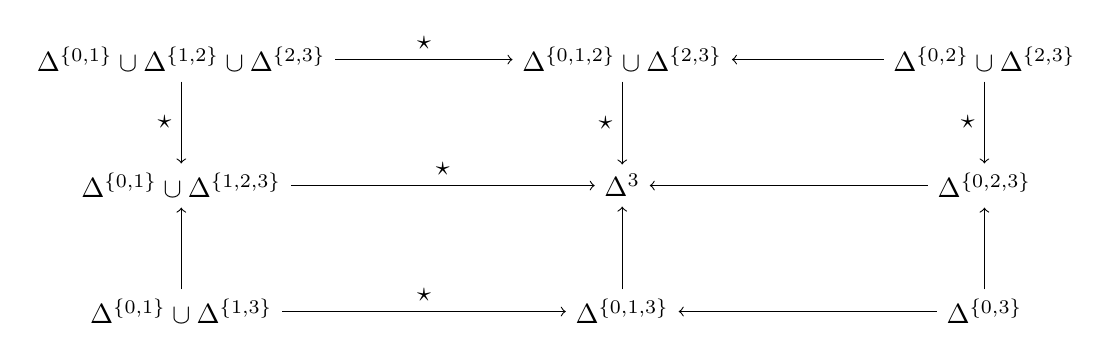
\begin{tikzpicture}
  \node (a1) at (0,0)
    {$\Delta^{\{0,1\}} \cup \Delta^{\{1,2\}} \cup \Delta^{\{2,3\}}$};
  \node (a2) at (5.6,0) {$\Delta^{\{0,1,2\}} \cup \Delta^{\{2,3\}}$};
  \node (a3) at (10.2,0) {$\Delta^{\{0,2\}} \cup \Delta^{\{2,3\}}$};
  \node (b1) at (0,-1.6) {$\Delta^{\{0,1\}} \cup \Delta^{\{1,2,3\}}$};
  \node (b2) at (5.6,-1.6) {$\Delta^{3}$};
  \node (b3) at (10.2,-1.6) {$\Delta^{\{0,2,3\}}$};
  \node (c1) at (0,-3.2) {$\Delta^{\{0,1\}} \cup \Delta^{\{1,3\}}$};
  \node (c2) at (5.6,-3.2) {$\Delta^{\{0,1,3\}}$};
  \node (c3) at (10.2,-3.2) {$\Delta^{\{0,3\}}$};
  \draw[->] (a1) -- node[above] {$\star$} (a2);
  \draw[->] (a3) -- (a2);
  \draw[->] (b1) -- node[above] {$\star$} (b2);
  \draw[->] (b3) -- (b2);
  \draw[->] (c1) -- node[above] {$\star$} (c2);
  \draw[->] (c3) -- (c2);
  \draw[->] (a1) -- node[left] {$\star$} (b1);
  \draw[->] (a2) -- node[left] {$\star$} (b2);
  \draw[->] (a3) -- node[left] {$\star$} (b3);
  \draw[->] (c1) -- (b1);
  \draw[->] (c2) -- (b2);
  \draw[->] (c3) -- (b3);
\end{tikzpicture}
\end{center}
并证明所有标有 $\star$ 的映射都是\trInnerAnodyne{}的。
\end{exercise}

\begin{exercise}\label{ex:homotopy-commutative-mapping-diagram}
设 $f\colon \mathcal{C} \to \mathcal{D}$ 是∞-\trCategories{}之间的一个\trFunctor{}。设
$a\colon x \to x'$ 与 $b\colon y \to y'$ 是 $\mathcal{C}$ 中的\trMorphism{}。证明：
存在一个由 \trKanComplex{}组成的同伦交换图表
\begin{center}
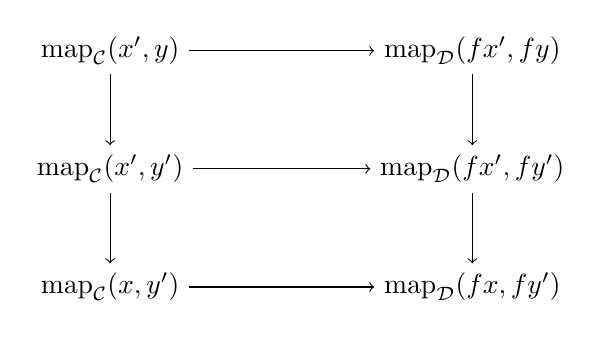
\begin{tikzpicture}
  \node (a) at (0,0) {$\mathrm{map}_{\mathcal{C}}(x', y)$};
  \node (b) at (4.6,0) {$\mathrm{map}_{\mathcal{D}}(fx', fy)$};
  \node (c) at (0,-1.5) {$\mathrm{map}_{\mathcal{C}}(x', y')$};
  \node (d) at (4.6,-1.5) {$\mathrm{map}_{\mathcal{D}}(fx', fy')$};
  \node (e) at (0,-3.0) {$\mathrm{map}_{\mathcal{C}}(x, y')$};
  \node (ff) at (4.6,-3.0) {$\mathrm{map}_{\mathcal{D}}(fx, fy')$};
  \draw[->] (a) -- (b);
  \draw[->] (c) -- (d);
  \draw[->] (e) -- (ff);
  \draw[->] (a) -- (c);
  \draw[->] (c) -- (e);
  \draw[->] (b) -- (d);
  \draw[->] (d) -- (ff);
\end{tikzpicture}
\end{center}
它由与 $a$（相应地 $fa$）的前合成、以及与 $b$（相应地 $fb$）的后合成所诱导。
由此推出：存在一个从 $\mathrm{Cat}^{1}_{\infty}$（∞-\trCategories{}的
$1$-\trCategory{}）到 $\mathrm{Cat}_{\pi(\mathrm{Kan})}$（充实于\trKanComplex{}的%
\trHomotopyCategory{}中的\trCategories{}构成的\trCategory{}）的典范\trFunctor{}%
$F$，其中 $F(\mathcal{C})$ 与 $\mathcal{C}$ 拥有相同的\trObject{}，而从 $x$ 到 $y$
的 hom 对象由 $\mathrm{map}_{\mathcal{C}}(x, y)$ 在 $\pi(\mathrm{Kan})$ 中的像给出。
\end{exercise}

\begin{exercise}\label{ex:join-simplex-cones}
证明 $[n] \star [m] = [n + m + 1]$。此外，证明
$\mathcal{C} \star [0] = \mathcal{C}^{\rhd}$ 且
$[0] \star \mathcal{C} = \mathcal{C}^{\lhd}$。
\end{exercise}

\begin{exercise}\label{ex:nerve-join}
证明：对\trCategories{} $\mathcal{C}$ 与 $\mathcal{D}$，我们有
$\mathrm{N}(\mathcal{C}) \star \mathrm{N}(\mathcal{D}) \cong \mathrm{N}(\mathcal{C} \star \mathcal{D})$。
特别地，证明存在典范同构
$\Delta^i \star \Delta^j \cong \Delta^{i+1+j}$。
\end{exercise}

\begin{exercise}\label{ex:join-not-colimit}
作为\trFunctor{} $\mathrm{sSet} \to \mathrm{sSet}$，\trFunctor{} $X \star -$ 与
$- \star X$ 保持\trPushout{}。找一个不被 $X \star -$ 保持的\trColimit{}的例子。
\end{exercise}

\begin{exercise}\label{ex:slice-join-lifting-bijection}
证明：切片／联伴随在如下图式之类的提升问题与
\begin{center}
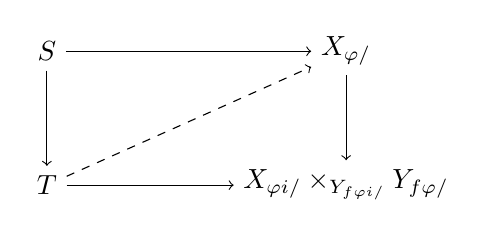
\begin{tikzpicture}
  \node (S) at (0,0) {$S$};
  \node (X) at (3.8,0) {$X_{\varphi/}$};
  \node (T) at (0,-1.7) {$T$};
  \node (B) at (3.8,-1.7)
    {$X_{\varphi i/} \times_{Y_{f\varphi i/}} Y_{f\varphi/}$};
  \draw[->] (S) -- (X);
  \draw[->] (S) -- (T);
  \draw[->] (X) -- (B);
  \draw[->] (T) -- (B);
  \draw[->,dashed] (T) -- (X);
\end{tikzpicture}
\end{center}
如下图式之类的提升问题之间，诱导一个双射：
\begin{center}
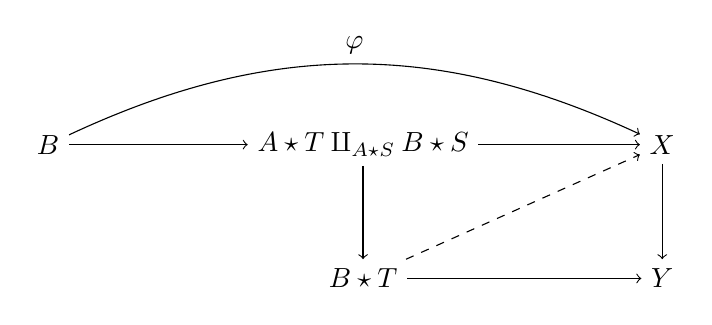
\begin{tikzpicture}
  \node (B) at (0,0) {$B$};
  \node (M) at (4.0,0) {$A \star T \amalg_{A \star S} B \star S$};
  \node (X) at (7.8,0) {$X$};
  \node (BT) at (4.0,-1.7) {$B \star T$};
  \node (Y) at (7.8,-1.7) {$Y$};
  \draw[->] (B) -- (M);
  \draw[->] (M) -- (X);
  \draw[->] (M) -- (BT);
  \draw[->] (BT) -- (Y);
  \draw[->] (X) -- (Y);
  \draw[->,dashed] (BT) -- (X);
  \draw[->] (B) to[bend left=25] node[above] {$\varphi$} (X);
\end{tikzpicture}
\end{center}
\end{exercise}

\begin{exercise}\label{ex:join-horn-computation}
证明
\[
\Lambda^n_j \star \Delta^m \cup \Delta^n \star \partial\Delta^m
= \Lambda^{n+1+m}_j
\]
与
\[
\partial\Delta^m \star \Delta^n \cup \Delta^m \star \Lambda^n_j
= \Lambda^{n+1+m}_{m+1+j}.
\]
为此，请显式地确定 $\Delta^{n+1+m}$ 的下列子单纯集：
\begin{enumerate}[label=(\arabic*)]
  \item $\partial\Delta^n \star \Delta^m$
  \item $\Lambda^n_j \star \Delta^m$
  \item $\Delta^m \star \partial\Delta^n$
  \item $\Delta^m \star \Lambda^n_j$
\end{enumerate}
\end{exercise}

\begin{exercise}\label{ex:slice-under-over-fibration}
对∞-\trCategory{} $\mathcal{C}$ 中的一个\trObject{} $x$，证明典范映射
$\mathcal{C}_{x/} \to \mathcal{C}$ 是\trLeftFibration{}，而
$\mathcal{C}_{/x} \to \mathcal{C}$ 是\trRightFibration{}。
\end{exercise}

\begin{exercise}\label{ex:slice-under-not-left-fibration}
证明：对一般\trSimplicialSet{} $X$ 的一个\trObject{} $x$，典范映射
$X_{x/} \to X$ 一般不是\trLeftFibration{}。
\end{exercise}

\begin{exercise}\label{ex:inner-anodyne-iso}
证明：\trInnerFibration{} $f\colon X \to Y$ 是\trInnerAnodyne{}的，当且仅当它是一个同构。
\end{exercise}

\begin{exercise}\label{ex:point-not-inner-anodyne}
证明 $\Delta^0 \to J$ 不是\trInnerAnodyne{}的。
\end{exercise}

\begin{exercise}\label{ex:left-right-anodyne-intersection}
证明：\trLeftAnodyne{}映射与\trRightAnodyne{}映射之交严格包含\trInnerAnodyne{}映射。
\end{exercise}

\begin{exercise}\label{ex:conservative-homotopy-categories}
证明：∞-\trCategories{}之间的\trFunctor{} $F\colon \mathcal{C} \to \mathcal{D}$ 是%
\trConservative{}，当且仅当诸\trHomotopyCategory{}之间的诱导\trFunctor{}%
$hF\colon h\mathcal{C} \to h\mathcal{D}$ 是\trConservative{}。此外，证明典范%
\trFunctor{} $\mathcal{C} \to \mathrm{N}(h\mathcal{C})$ 是\trConservative{}。
\end{exercise}

\begin{exercise}\label{ex:conservative-pullback}
证明：\trFunctor{} $p\colon \mathcal{C} \to \mathcal{D}$ 是\trConservative{}，当且仅当
下图是一个\trPullback{}：
\begin{center}
\begin{tikzpicture}
  \node (a) at (0,0) {$\mathcal{C}^{\simeq}$};
  \node (b) at (2.8,0) {$\mathcal{C}$};
  \node (c) at (0,-1.6) {$\mathcal{D}^{\simeq}$};
  \node (d) at (2.8,-1.6) {$\mathcal{D}$};
  \draw[->] (a) -- (b);
  \draw[->] (a) -- (c);
  \draw[->] (b) -- (d);
  \draw[->] (c) -- (d);
\end{tikzpicture}
\end{center}
\end{exercise}

\begin{exercise}\label{ex:inner-fibration-isofibration}
证明：∞-\trCategories{}之间的\trInnerFibration{} $\mathcal{C} \to \mathcal{D}$ 是一个%
\trIsofibration{}，当且仅当诱导\trFunctor{}%
$\mathrm{N}(h\mathcal{C}) \to \mathrm{N}(h\mathcal{D})$ 是一个\trIsofibration{}。
\end{exercise}

\begin{exercise}\label{ex:isofibration-op}
证明：∞-\trCategories{}之间的\trFunctor{} $\mathcal{C} \to \mathcal{D}$ 是一个%
\trIsofibration{}，当且仅当 $\mathcal{C}^{\mathrm{op}} \to \mathcal{D}^{\mathrm{op}}$
是一个\trIsofibration{}。
\end{exercise}

\begin{exercise}\label{ex:full-subcat-isofibration}
设 $\mathcal{C}_0 \subseteq \mathcal{C}$ 是一个满子\trCategory{}。证明：包含
$\mathcal{C}_0 \to \mathcal{C}$ 是\trIsofibration{}，若 $\mathcal{C}_0$ 对
$\mathcal{C}$ 中的\trEquivalence{}封闭，也就是说，若 $x \in \mathcal{C}_0$ 而
$y \in \mathcal{C}$ 等价于 $x$，则 $y$ 也在 $\mathcal{C}_0$ 中。
\end{exercise}

\begin{exercise}\label{ex:slice-joyal-equivalence}
证明：若 $f\colon x \to y$ 是一个\trEquivalence{}，则映射
$\mathcal{C}_{/x} \to \mathcal{C}_{/y}$ 与 $\mathcal{C}_{y/} \to \mathcal{C}_{x/}$
是\trJoyalEquivalence{}。
\end{exercise}

\begin{exercise}\label{ex:conservative-not-rlp}
证明：存在∞-\trCategories{}之间的一个\trFunctor{} $f\colon \mathcal{C} \to \mathcal{D}$，
它是\trConservative{}，但不满足对 $\Delta^1 \to J$ 的\trRightLiftingProperty{}。
提示：考虑映射 $J \to \mathcal{S}(|J|)$。
\end{exercise}

\begin{exercise}\label{ex:left-fibration-kan}
证明：\trLeftFibration{} $p\colon \mathcal{C} \to \mathcal{D}$ 是 \trKanFibration{}，
只要 $\mathcal{D}$ 是\trInfinityGroupoid{}。
\end{exercise}

\begin{exercise}\label{ex:isofibration-saturated}
设 $p\colon \mathcal{C} \to \mathcal{D}$ 是一个\trIsofibration{}。证明：由使得诱导映射
\[
\mathcal{C}^{L} \to \mathcal{C}^{K} \times_{\mathcal{D}^{K}} \mathcal{D}^{L}
\]
仍是\trIsofibration{}的全部\trMonomorphism{} $K \to L$ 组成的集合是一个%
\trSaturatedSet。
\end{exercise}

\begin{exercise}\label{ex:three-for-two}
证明：由\trEssentiallySurjective{}且\trFullyFaithful{}\trFunctor{}组成的类满足%
\trThreeForTwoProperty{}。
\end{exercise}

\begin{exercise}\label{ex:joyal-equivalence-core}
设 $f\colon \mathcal{C} \to \mathcal{D}$ 是一个\trJoyalEquivalence{}。证明：限制映射
$\mathcal{C}^{\simeq} \to \mathcal{D}^{\simeq}$ 也是一个\trJoyalEquivalence{}。
\end{exercise}

\begin{exercise}\label{ex:naturally-equivalent-functors}
证明：两个\trFunctor{} $f, g\colon \mathcal{C} \to \mathcal{D}$ 是自然等价的，当且仅当
$f$ 与 $g$ 表示 $\pi_0(\mathrm{Fun}(\mathcal{C}, \mathcal{D})^{\simeq})$ 中的同一个
元素。
\end{exercise}

\begin{exercise}\label{ex:joyal-equivalence-h}
证明：\trJoyalEquivalence{} $f\colon \mathcal{C} \to \mathcal{D}$ 诱导通常%
\trCategories{}的一个\trEquivalence{} $h\mathcal{C} \to h\mathcal{D}$。
\end{exercise}

\begin{exercise}\label{ex:joyal-equivalence-fun}
证明：∞-\trCategories{}之间的\trFunctor{} $f\colon \mathcal{C} \to \mathcal{D}$ 是一个%
\trJoyalEquivalence{}，当且仅当对每个\trSimplicialSet{} $K$，诱导映射
\[
f_{*}\colon \mathrm{Fun}(K, \mathcal{C}) \to \mathrm{Fun}(K, \mathcal{D})
\]
是一个\trJoyalEquivalence{}。
\end{exercise}

\begin{exercise}\label{ex:nerve-inner-anodyne-iso}
设 $F\colon \mathcal{C} \to \mathcal{D}$ 是通常\trCategories{}之间的一个\trFunctor{}。
证明：\trNerve{}上的诱导映射是\trInnerAnodyne{}的，当且仅当 $F$ 是一个同构。
\end{exercise}

\begin{exercise}\label{ex:saturated-localization}
设 $\mathcal{C}$ 是一个∞-\trCategory{}，$S$ 是 $\mathcal{C}$ 的一个\trMorphism{}集。
若 $S$ 与 $\bar{S}$（即在\trFunctor{} $\mathcal{C} \to \mathcal{C}[S^{-1}]$ 下被送到%
\trEquivalence{}的全部\trMorphism{}之集）重合，则称 $S$ 为\emph{\trSaturated{}}。
证明：
\begin{enumerate}[label=(\arabic*)]
  \item 若 $S \subseteq T$ 且 $T$ 是\trSaturated{}，则 $\bar{S} \subseteq T$；
  \item $\mathcal{C}$ 的两个\trMorphism{}集 $S$ 与 $T$ 给出\trJoyalEquivalence{}的%
        \trLocalization{}（与从 $\mathcal{C}$ 出发的映射相容），当且仅当
        $\bar{S} = \bar{T}$。
\end{enumerate}
\end{exercise}

\begin{exercise}\label{ex:iterated-localization}
证明或否证下述诸陈述：
\begin{enumerate}[label=(\arabic*)]
  \item 对每个∞-\trCategory{} $\mathcal{C}$、$\mathcal{C}$ 的一个\trMorphism{}集 $S$
        与 $\mathcal{C}[S^{-1}]$ 的一个\trMorphism{}集 $T$，\trFunctor{}%
        $\mathcal{C} \to \mathcal{C}[S^{-1}][T^{-1}]$ 是 $\mathcal{C}$ 的一个%
        \trLocalization{}。
  \item 对每个∞-\trCategory{} $\mathcal{C}$、$\mathcal{C}$ 的一个\trMorphism{}集 $S$
        与 $\mathcal{C}$ 的一个\trMorphism{}集 $T$，\trFunctor{}%
        $\mathcal{C} \to \mathcal{C}[S^{-1}][T^{-1}]$ 是 $\mathcal{C}$ 的一个%
        \trLocalization{}。这里，我们沿典范\trFunctor{}%
        $\mathcal{C} \to \mathcal{C}[S^{-1}]$ 把 $\mathcal{C}$ 的\trMorphism{}%
        视为 $\mathcal{C}[S^{-1}]$ 的\trMorphism{}。
\end{enumerate}
\end{exercise}

\begin{exercise}\label{ex:initial-localization-ordinary}
设 $\mathcal{C}$ 是一个通常\trCategory{}，$S$ 是一个\trMorphism{}集。证明
$\mathcal{C} \to h\mathcal{C}[S^{-1}]$ 是在把 $S$ 送到同构的通常\trCategories{}之间、
初始的\trFunctor{} $\mathcal{C} \to \mathcal{D}$（至多差一个自然同构）。
\end{exercise}

\begin{exercise}\label{ex:zigzag-calculus-of-fractions}
设 $\mathcal{C}$ 是一个通常\trCategory{}，$S$ 是一个\trMorphism{}集。证明
$h\mathcal{C}[S^{-1}]$ 中的每个\trMorphism{}都可以由 $\mathcal{C}$ 中\trMorphism{}的
一个之字形链（zig zag）来表示，使得指向错误方向的那些映射都含于 $S$。
\end{exercise}

\begin{exercise}\label{ex:pushout-groupoid}
设 $\mathcal{C}$ 是一个通常\trCategory{}。考虑\trCategories{}的一个\trPushout{}%
\begin{center}
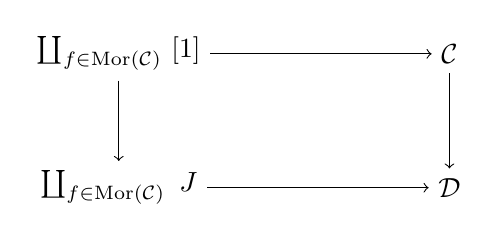
\begin{tikzpicture}
  \node (a) at (0,0)
    {$\coprod_{f \in \mathrm{Mor}(\mathcal{C})}\ [1]$};
  \node (b) at (4.2,0) {$\mathcal{C}$};
  \node (c) at (0,-1.7)
    {$\coprod_{f \in \mathrm{Mor}(\mathcal{C})}\ J$};
  \node (d) at (4.2,-1.7) {$\mathcal{D}$};
  \draw[->] (a) -- (b);
  \draw[->] (a) -- (c);
  \draw[->] (b) -- (d);
  \draw[->] (c) -- (d);
\end{tikzpicture}
\end{center}
其中 $\mathrm{Mor}(\mathcal{C})$ 表示 $\mathcal{C}$ 的全部\trMorphism{}之集。证明
$\mathcal{D}$ 是一个\trGroupoid{}。
\end{exercise}

\begin{exercise}\label{ex:unit-map-singular}
在本练习中，你可以使用如下事实：对任意 \trKanComplex{} $K$，单位映射
$K \to \mathcal{S}(|K|)$ 是一个\trHomotopyEquivalence{}。回顾：\trSimplicialSet{}的
一个映射是\trWeakEquivalence{}，如果它的\trGeometricRealization{}是一个%
\trHomotopyEquivalence{}；并设 $X$ 是一个\trSimplicialSet{}。证明或否证下述诸陈述：
\begin{enumerate}[label=(\arabic*)]
  \item 单位映射 $X \to \mathcal{S}(|X|)$ 是一个\trMonomorphism{}。
  \item 单位映射 $X \to \mathcal{S}(|X|)$ 是一个\trWeakEquivalence{}。
  \item 单位映射 $X \to \mathcal{S}(|X|)$ 是\trAnodyne{}的。
\end{enumerate}
\end{exercise}

\begin{exercise}\label{ex:localize-all-morphisms}
设 $\mathcal{C}$ 是一个∞-\trCategory{}，并设 $\mathcal{C} \to \mathcal{S}(|\mathcal{C}|)$
是伴随 $(\mathcal{S}, |{-}|)$ 的单位映射。证明这是 $\mathcal{C}$ 沿全部\trMorphism{}%
的一个\trLocalization{}。
\end{exercise}

\begin{exercise}\label{ex:path-fibration-functorial}
证明：∞-\trCategories{}之间的\trFunctor{} $f\colon \mathcal{C} \to \mathcal{D}$ 的
分解 $\mathcal{C} \to P(f) \to \mathcal{D}$ 是函子性的，也就是说，对每个实线交换图表
\begin{center}
\begin{tikzpicture}
  \node (a) at (0,0) {$\mathcal{C}$};
  \node (b) at (3.2,0) {$P(f)$};
  \node (c) at (6.4,0) {$\mathcal{D}$};
  \node (d) at (0,-1.6) {$\mathcal{C}'$};
  \node (e) at (3.2,-1.6) {$P(f')$};
  \node (ff) at (6.4,-1.6) {$\mathcal{D}'$};
  \draw[->] (a) -- (b);
  \draw[->] (b) -- (c);
  \draw[->] (d) -- (e);
  \draw[->] (e) -- (ff);
  \draw[->] (a) -- (d);
  \draw[->] (c) -- (ff);
  \draw[->,dashed] (b) -- (e);
\end{tikzpicture}
\end{center}
都存在一条虚箭头，使两个小方块都交换。
\end{exercise}

\begin{exercise}\label{ex:pushout-joyal-equivalence}
考虑\trSimplicialSet{}的一个\trPushout{}图表
\begin{center}
\begin{tikzpicture}
  \node (a) at (0,0) {$X$};
  \node (b) at (2.6,0) {$Y$};
  \node (c) at (0,-1.6) {$X'$};
  \node (d) at (2.6,-1.6) {$Y'$};
  \draw[->] (a) -- (b);
  \draw[->] (a) -- (c);
  \draw[->] (b) -- (d);
  \draw[->] (c) -- (d);
\end{tikzpicture}
\end{center}
其中 $X \to X'$ 是\trMonomorphism{}，而 $X \to Y$ 是\trJoyalEquivalence{}。证明映射
$X' \to Y'$ 也是\trJoyalEquivalence{}。
\end{exercise}

\begin{exercise}\label{ex:joyal-equivalence-coproduct-product}
设 $X \to X'$ 与 $Y \to Y'$ 是\trSimplicialSet{}之间的\trJoyalEquivalence{}。证明映射
$X \amalg Y \to X' \amalg Y'$ 与 $X \times Y \to X' \times Y'$ 都是%
\trJoyalEquivalence{}。
\end{exercise}

\begin{exercise}\label{ex:joyal-equivalence-retract-saturated}
证明：
\begin{enumerate}[label=(\arabic*)]
  \item \trJoyalEquivalence{}的\trRetract{}是\trJoyalEquivalence{}。
  \item 由同时是\trJoyalEquivalence{}的\trMonomorphism{}组成的集合是\trSaturated{}。
\end{enumerate}
证明或否证：由\trJoyalEquivalence{}组成的集合是\trSaturated{}。
\end{exercise}

\begin{exercise}\label{ex:pre-inverse}
回顾：称映射 $f\colon X \to Y$ 容许一个\emph{前逆}（pre-inverse），如果存在映射
$g\colon Y \to X$、$\tau\colon \Delta^1 \to \mathrm{Hom}(X, X)$ 与
$\tau'\colon \Delta^1 \to \mathrm{Hom}(Y, Y)$，使得
\begin{enumerate}[label=(\arabic*)]
  \item $\tau_{\varepsilon} = \mathrm{id}_X$ 且 $\tau_{1+\varepsilon} = gf$，其中
        $\varepsilon \in \{0, 1\} \cong \mathbb{Z}/2$；
  \item $\tau'_{\varepsilon} = \mathrm{id}_Y$ 且 $\tau'_{1+\varepsilon} = fg$，其中
        同样 $\varepsilon \in \{0, 1\} \cong \mathbb{Z}/2$；
  \item 对 $X$ 的所有\trObject{} $x$，\trMorphism{} $\tau(x)\colon \Delta^1 \to X$
        表示 $X$ 的一条退化边；对 $Y$ 的所有\trObject{} $y$，
        $\tau'(y)\colon \Delta^1 \to Y$ 表示 $Y$ 的一条退化边。
\end{enumerate}
证明：容许前逆的映射 $f\colon X \to Y$ 是\trJoyalEquivalence{}。
\end{exercise}

\begin{exercise}\label{ex:inner-fibration-trivial}
设 $p\colon \mathcal{C} \to \mathcal{D}$ 是∞-\trCategories{}之间的一个%
\trInnerFibration{}，它在 $0$-\trSimplex{}上诱导满射，并且是\trJoyalEquivalence{}。
证明 $p$ 是\trTrivialFibration{}。
\end{exercise}

\begin{exercise}\label{ex:join-retract-fat-join}
证明：对任意两个\trSimplicialSet{}，$X \star Y$ 是 $X \diamond Y$ 的一个\trRetract{}。
\end{exercise}

\begin{exercise}\label{ex:realization-hom-homotopy-equivalence}
证明典范映射
\[
|\underline{\mathrm{Hom}}(A, B)| \longrightarrow \mathrm{map}(|A|, |B|)
\]
是一个\trHomotopyEquivalence{}。你可以使用如下事实：单位映射
$A \to \mathcal{S}(|A|)$ 与余单位映射 $|\mathcal{S}(X)| \to X$ 都是%
\trWeakEquivalence{}。
\end{exercise}

下面诸练习的目标，是对「\trAnodyneMap{}恰是那些作为\trWeakEquivalence{}的%
\trMonomorphism{}」这一事实给出一个（近乎完整的）证明。更精确地说，我们将证明：
该事实由下述陈述推出。设 $p\colon X \to Y$ 是一个 \trKanFibration{}。那么 $p$ 有
一个分解
\[
X \xrightarrow{\ \alpha\ } Z \xrightarrow{\ \beta\ } Y
\]
其中 $\beta$ 是\trTrivialFibration{}（也就是说，它对\trMonomorphism{}具有%
\trRightLiftingProperty{}），而 $\alpha$ 是一个极小纤维化（minimal fibration）。
在这一语境中，我们需要关于极小纤维化的下列事实：
\begin{itemize}
  \item 极小纤维化是 \trKanFibration{}。
  \item 极小纤维化 $\alpha\colon X \to Z$ 是局部平凡的（locally trivial），也就是
        说，对每个\trSimplex{} $\Delta^n \to Z$，拉回得到的纤维化（在 $\Delta^n$
        之上）同构于一个投影 $\Delta^n \times B \to \Delta^n$。
\end{itemize}

\begin{exercise}\label{ex:kan-fibration-contractible-fibres}
证明：\trKanFibration{} $p\colon X \to Y$ 是\trTrivialFibration{}，当且仅当它的诸%
\trFibre{}是\trContractible{}。提示：对有趣的方向，考虑提升问题
\begin{center}
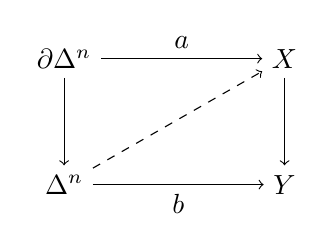
\begin{tikzpicture}
  \node (a) at (0,0) {$\partial\Delta^n$};
  \node (b) at (2.8,0) {$X$};
  \node (c) at (0,-1.6) {$\Delta^n$};
  \node (d) at (2.8,-1.6) {$Y$};
  \draw[->] (a) -- node[above] {$a$} (b);
  \draw[->] (a) -- (c);
  \draw[->] (b) -- (d);
  \draw[->] (c) -- node[below] {$b$} (d);
  \draw[->,dashed] (c) -- (b);
\end{tikzpicture}
\end{center}
为便于后续引用，令 $y = b(n)$。考虑由 $g(k, 0) = k$ 与 $g(k, 1) = n$ 确定的映射
$g\colon \Delta^n \times \Delta^1 \to \Delta^n$。证明映射
$\partial\Delta^n \times \{0\} \to \partial\Delta^n \times \Delta^1$ 是%
\trAnodyne{}的，
并利用 $g$ 得到一个映射
\[
\Delta^1 \to X^{\partial\Delta^n} \times_{Y^{\partial\Delta^n}} Y^{\Delta^n}
\]
它把 $0$ 送到原来的方块，而把 $1$ 送到方块
\begin{center}
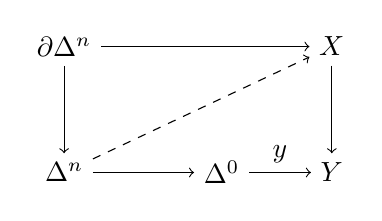
\begin{tikzpicture}
  \node (a) at (0,0) {$\partial\Delta^n$};
  \node (b) at (3.4,0) {$X$};
  \node (c) at (0,-1.6) {$\Delta^n$};
  \node (e) at (2.0,-1.6) {$\Delta^0$};
  \node (d) at (3.4,-1.6) {$Y$};
  \draw[->] (a) -- (b);
  \draw[->] (a) -- (c);
  \draw[->] (b) -- (d);
  \draw[->] (c) -- (e);
  \draw[->] (e) -- node[above] {$y$} (d);
  \draw[->,dashed] (c) -- (b);
\end{tikzpicture}
\end{center}
其中映射 $\Delta^0 \to Y$ 就是\trObject{} $y$。证明这个提升问题可解。最后，证明这
蕴含原来的提升问题也可解。
\end{exercise}

\begin{exercise}\label{ex:realization-serre-fibration}
在本练习中，我们将利用极小纤维化来证明：\trKanFibration{} $p\colon X \to Y$ 的%
\trGeometricRealization{}是一个 Serre 纤维化，也就是说，它对包含
$D^n \times \{0\} \to D^n \times D^1$ 具有\trRightLiftingProperty{}。这里，$D^n$
是 $n$ 维拓扑立方体。
\begin{enumerate}[label=(\arabic*)]
  \item 证明：极小纤维化的\trGeometricRealization{}是一个 Serre 纤维化，其纤维由
        该\trKanFibration{}之\trFibre{}的\trGeometricRealization{}给出。
  \item 证明：\trTrivialFibration{}的\trGeometricRealization{}是一个 Serre 纤维化。
\end{enumerate}
提示：对（1），证明局部平凡映射的几何实现也是局部平凡的；然后证明空间的局部平凡
映射是 Serre 纤维化。对（2），证明存在\trMonomorphism{} $X \to W$，其中 $W$ 是一个%
\trContractible{} \trKanComplex{}。考虑映射 $X \to W \times Y \to Y$。证明后者是%
\trTrivialFibration{}，并由此推出 $p$ 是 $W \times Y \to Y$ 的一个\trRetract{}。
\end{exercise}

\begin{exercise}\label{ex:kan-fibration-weak-equivalence-fibres}
证明：作为\trWeakEquivalence{}的\trKanFibration{} $p\colon X \to Y$ 具有%
\trContractible{}诸\trFibre{}。
\end{exercise}

\begin{exercise}\label{ex:mono-weak-equivalence-anodyne}
证明：\trMonomorphism{} $i\colon A \to B$ 是\trWeakEquivalence{}，当且仅当它是%
\trAnodyne{}的。
\end{exercise}

\begin{exercise}\label{ex:cocartesian-trivial-fibration}
证明：诸\trFibre{}都\trJoyalEquivalence{}于 $\Delta^0$ 的\trCocartesianFibration{}%
$p\colon X \to Y$ 是\trTrivialFibration{}。
\end{exercise}

\begin{exercise}\label{ex:poset-extension}
设 $P$ 是一个偏序集，$\mathcal{C}$ 是一个∞-\trCategory{}。设给定了一个函数
$f\colon P \to \mathrm{ob}(\mathcal{C})$，它具有下述性质：每当 $x \le y$ 是 $P$
中的元素时，映射空间 $\mathrm{map}_{\mathcal{C}}(fx, fy)$ 都是\trContractible{}。
\begin{enumerate}[label=(\arabic*)]
  \item 证明：存在一个在\trObject{}上延拓所给函数 $f$ 的\trFunctor{}%
        $F\colon P \to \mathcal{C}$。
  \item 证明：任意两个这样的延拓都是等价的。
\end{enumerate}
当然，（2）的「正确」版本是下述陈述：证明存在一个参数化所有可能延拓选择的%
\trContractible{}空间；也就是说，在\trPullback{}图表
\begin{center}
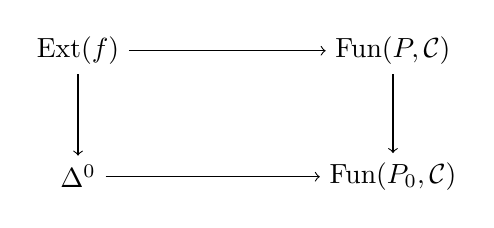
\begin{tikzpicture}
  \node (a) at (0,0) {$\mathrm{Ext}(f)$};
  \node (b) at (4.0,0) {$\mathrm{Fun}(P, \mathcal{C})$};
  \node (c) at (0,-1.6) {$\Delta^0$};
  \node (d) at (4.0,-1.6) {$\mathrm{Fun}(P_0, \mathcal{C})$};
  \draw[->] (a) -- (b);
  \draw[->] (a) -- (c);
  \draw[->] (b) -- (d);
  \draw[->] (c) -- (d);
\end{tikzpicture}
\end{center}
中，\trSimplicialSet{} $\mathrm{Ext}(f)$ 是一个\trContractible{} \trKanComplex{}。
能否把 $P$ 换成任意一个 $1$-\trCategory{}并得到同样的结果？
\end{exercise}

\begin{exercise}\label{ex:sequential-functor}
设 $\mathcal{C}$ 是一个∞-\trCategory{}，并对每个 $i \ge 0$ 考虑 $\mathcal{C}$ 中%
\trObject{}之间的一个\trMorphism{} $x_i \to x_{i+1}$。证明这些映射装配成一个%
\trFunctor{} $\mathbb{N} \to \mathcal{C}$。
\end{exercise}

\begin{exercise}\label{ex:isofibration-trivial-fibres}
证明或否证：∞-\trCategories{}之间的\trIsofibration{} $p\colon \mathcal{C} \to \mathcal{D}$
是\trTrivialFibration{}，当且仅当它的诸\trFibre{}都\trJoyalEquivalence{}于
$\Delta^0$。
\end{exercise}

\begin{exercise}\label{ex:p-cocartesian-over-point}
设 $\mathcal{C}$ 是一个∞-\trCategory{}，并考虑\trInnerFibration{}%
$p\colon \mathcal{C} \to \Delta^0$。证明 $\mathcal{C}$ 中的一个\trMorphism{} $f$
是 $p$-(余)笛卡尔的，当且仅当 $f$ 是一个\trEquivalence{}。
\end{exercise}

\begin{exercise}\label{ex:homotopy-cartesian-square-invariant}
证明：若在两个∞-\trCategories{}的方块之间给出一个态射，其中每个比较映射都是%
\trJoyalEquivalence{}，则其中一个方块是\trHomotopyCartesian{}，当且仅当另一个方块也是。
\end{exercise}

\begin{exercise}\label{ex:pullback-cartesian-fibration}
设有\trPullback{}图表
\begin{center}
\begin{tikzpicture}
  \node (a) at (0,0) {$X'$};
  \node (b) at (2.8,0) {$X$};
  \node (c) at (0,-1.6) {$Y'$};
  \node (d) at (2.8,-1.6) {$Y$};
  \draw[->] (a) -- node[above] {} (b);
  \draw[->] (a) -- node[left] {$p'$} (c);
  \draw[->] (b) -- node[right] {$p$} (d);
  \draw[->] (c) -- (d);
\end{tikzpicture}
\end{center}
其中映射 $p$ 是一个（余）笛卡尔纤维化。证明映射 $p'$ 也是一个（余）笛卡尔纤维化。
\end{exercise}

\begin{exercise}\label{ex:p-prime-cocartesian-locally-cocartesian}
设 $p\colon X \to S$ 是\trSimplicialSet{}的一个\trInnerFibration{}，$f\colon x \to y$
是 $X$ 中的一条边。设 $f$ 是 $p'$-余笛卡尔的，其中 $p'$ 由下述\trPullback{}给出：
\begin{center}
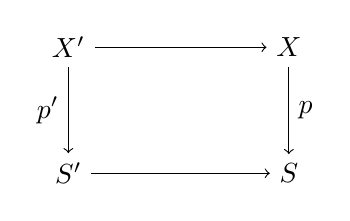
\begin{tikzpicture}
  \node (a) at (0,0) {$X'$};
  \node (b) at (2.8,0) {$X$};
  \node (c) at (0,-1.6) {$S'$};
  \node (d) at (2.8,-1.6) {$S$};
  \draw[->] (a) -- (b);
  \draw[->] (a) -- node[left] {$p'$} (c);
  \draw[->] (b) -- node[right] {$p$} (d);
  \draw[->] (c) -- (d);
\end{tikzpicture}
\end{center}
证明 $f$ 是局部余笛卡尔的。
\end{exercise}

\begin{exercise}\label{ex:prove-lemma-3-2-7}
证明第 3 章中的\cref{lem:locally-cocartesian-two-out-of-three}。
\end{exercise}

\begin{exercise}\label{ex:quotient-inner-fibration}
考虑\trSimplicialSet{} $S = \Delta^2/\Delta^{\{0,1\}}$ 与典范映射
$p\colon \Delta^{\{0,2\}} \to S$。证明图表
\begin{center}
\begin{tikzpicture}
  \node (a) at (0,0) {$\Lambda^2_0$};
  \node (b) at (3.4,0) {$\Delta^{\{0,2\}}$};
  \node (c) at (0,-1.6) {$\Delta^2$};
  \node (d) at (3.4,-1.6) {$S$};
  \draw[->] (a) -- node[above] {$f$} (b);
  \draw[->] (a) -- (c);
  \draw[->] (b) -- (d);
  \draw[->] (c) -- node[below] {$c$} (d);
\end{tikzpicture}
\end{center}
是一个\trPullback{}，其中 $c$ 是典范投影。然后接着证明：
\begin{enumerate}[label=(\arabic*)]
  \item $p$ 是一个\trInnerFibration{}。
  \item 边 $f|_{\Delta^{\{0,1\}}}$ 是退化的，但不是 $p$-余笛卡尔的。
\end{enumerate}
\end{exercise}

\begin{exercise}\label{ex:flat-sharp-adjunctions}
证明：诸\trFunctor{} $(-)^{\flat}, (-)^{\sharp}\colon \mathrm{sSet} \to \mathrm{sSet}_+$
与诸\trFunctor{} $u, m\colon \mathrm{sSet}_+ \to \mathrm{sSet}$ 参与了多种伴随。这里，
$u$ 是\trForgetfulFunctor{}，而 $m$ 是把\trMarkedSimplicialSet{} $(X, S)$ 送到包含
$S$ 的最小子单纯集 $X_0 \subseteq X$ 的那个\trFunctor{}。
\end{exercise}

\begin{exercise}\label{ex:fun-mcc-core}
设 $p\colon \E \to \mathcal{C}$ 是一个\trCocartesianFibration{}，$K$ 是一个%
\trMarkedSimplicialSet{}，并装备有映射 $f\colon K \to \mathcal{C}^{\sharp}$。考虑
$\mathrm{Fun}^{\mathrm{mcc}}_f(K, \E)$ 的、由那些对应的映射
$K \times \Delta^1 \to \E$ 是\trMarkedSimplicialSet{}的映射
$K \times (\Delta^1)^{\sharp} \to \E^{\natural}$ 的 $1$-\trSimplex{}组成的子∞-%
\trCategory{}；也就是说，我们只考虑那些在诸分量上\trPointwise{}为 $p$-余笛卡尔的函子变换。
证明这个子∞-\trCategory{}由 $\mathrm{Fun}^{\mathrm{mcc}}_f(K, \E)^{\simeq}$ 给出。
\end{exercise}

\begin{exercise}\label{ex:fun-cc-over-z}
证明：若 $K = \Delta^0$ 且 $f\colon \Delta^0 \to \mathcal{C}$ 挑出 $\mathcal{C}$ 的
一个\trObject{} $z$，则 $\mathrm{Fun}^{\mathrm{cc}}(K, \E) \cong \E$ 且
$\mathrm{Fun}^{\mathrm{cc}}_f(K, \E) \cong \E_z$。
\end{exercise}

\begin{exercise}\label{ex:map-flat-sharp}
设 $X \to Y$ 是一个\trCocartesianFibration{}，$f\colon K \to Y^{\sharp}$ 是%
\trMarkedSimplicialSet{}的映射。证明 $\mathrm{Map}^{\flat}_{f}(K, X^{\natural})$ 是一个
∞-\trCategory{}，而 $\mathrm{Map}^{\sharp}_{f}(K, X^{\natural})$ 是
$\mathrm{Map}^{\flat}_{f}(K, X^{\natural})$ 内部最大的子\trInfinityGroupoid{}。
\end{exercise}

\begin{exercise}\label{ex:flat-marked-equivalence}
证明：\trFunctor{} $(-)^{\flat}\colon \mathrm{sSet} \to \mathrm{sSet}_+$ 把%
\trJoyalEquivalence{}送到\trMarkedEquivalence{}。
\end{exercise}

\begin{exercise}\label{ex:marked-simplicial-enriched}
证明：\trMarkedSimplicialSet{}的\trCategory{}典范地充实于单纯集。
\end{exercise}

\begin{exercise}\label{ex:LF-preserves-colimits}
证明：第 3 章中的\cref{thm:initial-vertex-joyal-equivalence}的\trFunctor{}%
$LF\colon \mathrm{sSet} \to \mathrm{sSet}$ 保持\trColimit{}与\trMonomorphism{}。
\end{exercise}

\begin{exercise}\label{ex:initial-vertex-natural-transformation}
证明诸\trInitialVertexMap{}装配成一个\trNaturalTransformation{} $LF \Rightarrow \mathrm{id}$。
\end{exercise}

\begin{exercise}\label{ex:colim-joyal-equivalence-sequential}
设有交换图表
\begin{center}
\begin{tikzpicture}
  \node (a0) at (0,0) {$A_0$};
  \node (a1) at (2.6,0) {$A_1$};
  \node (a2) at (5.2,0) {$A_2$};
  \node (a3) at (7.6,0) {$\dots$};
  \node (b0) at (0,-1.6) {$B_0$};
  \node (b1) at (2.6,-1.6) {$B_1$};
  \node (b2) at (5.2,-1.6) {$B_2$};
  \node (b3) at (7.6,-1.6) {$\dots$};
  \draw[->] (a0) -- (a1);
  \draw[->] (a1) -- (a2);
  \draw[->] (a2) -- (a3);
  \draw[->] (b0) -- (b1);
  \draw[->] (b1) -- (b2);
  \draw[->] (b2) -- (b3);
  \draw[->] (a0) -- node[left] {$f_0$} (b0);
  \draw[->] (a1) -- node[left] {$f_1$} (b1);
  \draw[->] (a2) -- node[left] {$f_2$} (b2);
\end{tikzpicture}
\end{center}
其中诸映射 $f_i$ 都是\trJoyalEquivalence{}，而全部水平映射都是\trMonomorphism{}。
证明诱导映射 $f\colon A = \mathrm{colim}\, A_i \to \mathrm{colim}\, B_i = B$ 是一个%
\trJoyalEquivalence{}。
\end{exercise}

\begin{exercise}\label{ex:groupoid-op-equivalent}
证明：对\trInfinityGroupoid{} $X$，存在典范的\trJoyalEquivalence{}%
$X^{\mathrm{op}} \simeq X$。
\end{exercise}

\begin{exercise}\label{ex:delta-op-full}
证明\trFunctor{}%
$\mathrm{N}(\Delta^{\mathrm{op}}_{/\mathcal{C}}) \to \mathcal{C}$ 是满的，其意义是：
$\mathcal{C}$ 的每个\trMorphism{}都是该\trFunctor{}下某个\trMorphism{}的像。利用
这个结果证明：复合 $\mathcal{C} \to \mathrm{Cat}_{\infty}$ 在\trObject{}与%
\trMorphism{}上诱导出我们先前做过的那些构造。
\end{exercise}

\begin{exercise}\label{ex:cocartesian-pushforward-diagram}
设有\trCocartesianFibration{} $p\colon \E \to \mathcal{C}$。回顾：我们对每条边
$f\colon \Delta^1 \to \mathcal{C}$ 构造了一个\trFunctor{} $\E_x \times \Delta^1 \to \E$，
其在 $\E_x \times \{1\}$ 上的限制由 $f_!$ 给出。证明这个\trFunctor{}也可以等价地
通过考虑图表
\begin{center}
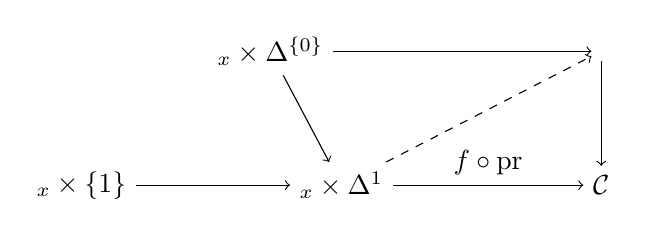
\begin{tikzpicture}
  \node (a) at (0,0) {$\E_x \times \Delta^{\{0\}}$};
  \node (b) at (4.2,0) {$\E$};
  \node (c) at (-2.4,-1.7) {$\E_x \times \{1\}$};
  \node (d) at (0.9,-1.7) {$\E_x \times \Delta^1$};
  \node (e) at (4.2,-1.7) {$\mathcal{C}$};
  \draw[->] (a) -- (b);
  \draw[->] (a) -- (d);
  \draw[->] (c) -- (d);
  \draw[->] (d) -- node[above] {$f \circ \mathrm{pr}$} (e);
  \draw[->] (b) -- (e);
  \draw[->,dashed] (d) -- (b);
\end{tikzpicture}
\end{center}
来构造，并证明存在一条具备上述全部性质的虚箭头。
\end{exercise}

\begin{exercise}\label{ex:cocartesian-family}
给定一个\trCocartesianFibration{} $\E \to \mathcal{C} \times \Delta^1$，构造一个与
到 $\mathcal{C}$ 的投影交换的\trFunctor{} $\E_0 \to \E_1$。这里，$\E_i$ 是沿包含
$\mathcal{C} \times \{i\} \to \mathcal{C} \times \Delta^1$ 拉回得到的%
\trCocartesianFibration{}。证明这个\trFunctor{}是余笛卡尔纤维化的一个态射。同样地，
对\trCocartesianFibration{} $\E \to \mathcal{C} \times \Delta^2$，构造∞-%
\trCategory{} $(\mathrm{Cat}_{\infty})_{/\mathcal{C}}$ 中的一个 $2$-%
\trSimplex{}。如果你有兴致，就把这一切对一般的 $n$（而非 $2$）做一遍。
\end{exercise}

\begin{exercise}\label{ex:inner-fibration-joyal-equivalence-fibrewise}
设 $p\colon \mathcal{C} \to \mathcal{D}$ 是∞-\trCategories{}之间的一个%
\trInnerFibration{}。假设对每个映射 $f\colon \Delta^1 \to \mathcal{D}$，诱导映射
$\Delta^1 \times_{\mathcal{D}} \mathcal{C} \to \Delta^1$ 都是\trJoyalEquivalence{}。
证明 $p$ 是\trJoyalEquivalence{}。
\end{exercise}

\begin{exercise}\label{ex:terminal-object-slice}
设 $\mathcal{C}$ 是一个∞-\trCategory{}，$x$ 是 $\mathcal{C}$ 的一个\trObject{}。
证明：由 $\Delta^0 \to \mathcal{C}_{/x}$ 所表示、伴随于由 $\mathrm{id}_x$ 给出的映射
$\Delta^0 \star \Delta^0 \to \mathcal{C}$ 的那个\trObject{}是一个%
\trTerminalObject{}。
\end{exercise}

\begin{exercise}\label{ex:initial-closed-under-equivalence}
设 $\mathcal{C}$ 是一个∞-\trCategory{}，$x$ 是 $\mathcal{C}$ 的一个\trInitialObject{}。
证明：若 $y$ 等价于 $x$，则 $y$ 在 $\mathcal{C}$ 中也是始的。
\end{exercise}

\begin{exercise}\label{ex:terminal-functor-values}
假设 $\mathcal{C}_{\mathrm{term}}$ 非空。证明 $\mathrm{Fun}(K, \mathcal{C})$ 的任何%
\trTerminalObject{}都在 $\mathcal{C}_{\mathrm{term}}$ 中取值。
\end{exercise}

\begin{exercise}\label{ex:fun-terminal-not-c}
证明：存在 $\mathcal{C}$ 与 $K$，使得 $\mathrm{Fun}(K, \mathcal{C})$ 拥有一个%
\trTerminalObject{}而 $\mathcal{C}$ 却没有。
\end{exercise}

\begin{exercise}\label{ex:twisted-arrow-not-right-fibration}
证明：存在\trSimplicialSet{} $X$，使得第 4 章中的\cref{def:twisted-arrow}的映射
$\mathrm{Tw}(X) \to X \times X^{\mathrm{op}}$ 不是一个\trRightFibration{}。
\end{exercise}

\begin{exercise}\label{ex:homotopy-cartesian-fully-faithful}
证明或否证：图表
\begin{center}
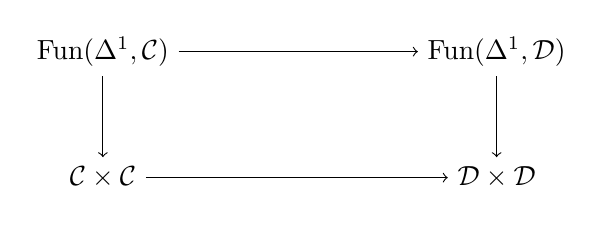
\begin{tikzpicture}
  \node (a) at (0,0) {$\mathrm{Fun}(\Delta^1, \mathcal{C})$};
  \node (b) at (5.0,0) {$\mathrm{Fun}(\Delta^1, \mathcal{D})$};
  \node (c) at (0,-1.6) {$\mathcal{C} \times \mathcal{C}$};
  \node (d) at (5.0,-1.6) {$\mathcal{D} \times \mathcal{D}$};
  \draw[->] (a) -- (b);
  \draw[->] (a) -- (c);
  \draw[->] (b) -- (d);
  \draw[->] (c) -- (d);
\end{tikzpicture}
\end{center}
是\trHomotopyCartesian{}，当且仅当 $f$ 是\trFullyFaithful{}。
\end{exercise}

\begin{exercise}\label{ex:colimit-equivalent-object}
设 $p\colon K \to \mathcal{C}$ 是一个图表。假设存在 $p$ 的一个余极限锥
$\tilde{p}$，其\trColimit{}为 $x \in \mathcal{C}$。设 $y$ 是 $\mathcal{C}$ 的一个
等价于 $x$ 的\trObject{}。证明 $y$ 也是 $p$ 的某个余极限锥的余极限。
\end{exercise}

\begin{exercise}\label{ex:slice-iso-adjoint}
设 $p\colon K \to \mathcal{C}$ 是一个图表，$q\colon I \to \mathcal{C}_{p/}$ 是另一个
图表。设 $\bar{q}\colon I \star K \to \mathcal{C}$ 是相联系的映射。证明存在同构
$(\mathcal{C}_{p/})_{q/} \cong \mathcal{C}_{\bar{q}/}$。同样地，证明存在同构
$(\mathcal{C}_{/p})_{q/} \cong (\mathcal{C}_{q'/})_{/p'}$，其中 $q'$ 是
$q\colon I \star K \to \mathcal{C}$\footnote{译注：原书此处作
「$q\colon I \star K \to \mathcal{C}$」，按本题开头 $q$ 之定义域为 $I$，
疑为 $\bar{q}$ 之误。} 到 $I$ 上的限制，而 $p'$ 伴随于 $\bar{q}$。
\end{exercise}

\begin{exercise}\label{ex:colimit-coequalizer}
设 $K$ 是两个\trMonomorphism{} $f, g\colon A \to B$ 的余等化子，并设
$F\colon K \to \mathcal{C}$ 是一个\trFunctor{}。假设 $F$ 在 $B$ 与 $A$ 上的限制都
容许\trColimit{}，且 $\mathcal{C}$ 容许余等化子。证明此时 $F$ 容许一个%
\trColimit{}。
\end{exercise}

\begin{exercise}\label{ex:preserves-small-colimits}
设 $F\colon \mathcal{C} \to \mathcal{D}$ 是∞-\trCategories{}之间的一个\trFunctor{}。
证明：$F$ 保持小\trColimit{}，当且仅当它保持小\trCoproduct{}与\trPushout{}%
（或余等化子）。
\end{exercise}

\begin{exercise}\label{ex:cofinal-coinitial-op}
证明：映射 $f\colon K \to L$ 是\trCofinal{}，当且仅当
$f^{\mathrm{op}}\colon K^{\mathrm{op}} \to L^{\mathrm{op}}$ 是\trCoinitial{}。
\end{exercise}

\begin{exercise}\label{ex:left-anodyne-no-cancellation}
证明：\trLeftAnodyne{}映射在\trMonomorphism{}之中不满足左消去性质（left cancellation
property）。
\end{exercise}

\begin{exercise}\label{ex:epsilon-natural-in-x}
设 $f\colon \mathcal{C} \to \mathcal{D}$ 与 $g\colon \mathcal{D} \to \mathcal{C}$
是\trFunctor{}。假设 $\varepsilon\colon fg \to \mathrm{id}$ 是一个%
\trNaturalTransformation{}。证明映射
\[
\mathrm{map}(x, g(y)) \to \mathrm{map}(f(x), f(g(y))) \to \mathrm{map}(f(x), y)
\]
在 $x$ 上是自然的。
\end{exercise}

\begin{exercise}\label{ex:right-anodyne-pullback-saturated}
证明：由沿任意\trLeftFibration{}的拉回仍是\trRightAnodyne{}的\trRightAnodyne{}映射
$i\colon A \to B$ 组成的集合是一个\trSaturatedSet，并且满足右消去性质（right-cancellation property）。
\end{exercise}

\begin{exercise}\label{ex:right-deformation-retract}
右形变收缩（right deformation retract）是一个\trMonomorphism{} $i\colon A \to B$，
使得存在一个\trRetraction{} $p\colon B \to A$ 与一个单纯同伦
$H\colon \Delta^1 \times B \to B$，满足 $H(0) = \mathrm{id}_B$、$H(1) = ip$，并且
其在 $\Delta^1 \times A$ 上的限制常值于 $A$ 的恒等。
\begin{enumerate}[label=(\arabic*)]
  \item 证明：对每个\trSimplicialSet{} $K$，映射 $\{1\} \times K \to \Delta^1 \times K$
        是一个右形变收缩。
  \item 证明：右形变收缩是\trRightAnodyne{}映射。
  \item 证明：右形变收缩沿\trLeftFibration{}的拉回仍是右形变收缩。
\end{enumerate}
\end{exercise}

\begin{exercise}\label{ex:proper-not-universally-proper}
给出一个\trProper{}（或\trSmooth{}）映射，但它不是\trUniversallyProper{}%
（或\trUniversallySmooth{}）的例子。
\end{exercise}

\begin{exercise}\label{ex:colimit-boundary-restriction}
设 $\mathcal{C}$ 是一个\trCocomplete{}∞-\trCategory{}，$F\colon \Delta^n \to \mathcal{C}$
是一个\trFunctor{}。计算限制 $\partial\Delta^n \to \Delta^n \to \mathcal{C}$ 的%
\trColimit{}。
\end{exercise}

\begin{exercise}\label{ex:cartesian-fibre-right-adjoint}
设 $p\colon \E \to \mathcal{D}$ 是一个\trCartesianFibration{}。证明典范映射
$\E_d \to \E_{d/}$ 容许一个\trRightAdjoint{}。由此推出：对\trCartesianFibration{}，
典范映射 $\E_d \to \E_{d/}$ 是一个\trWeakEquivalence{}。
\end{exercise}

\begin{exercise}\label{ex:fully-faithful-invertible}
证明：\trFullyFaithful{}且\trEssentiallySurjective{}\trFunctor{}是\trInvertible{}。
\end{exercise}

\begin{exercise}\label{ex:colimit-cocartesian-localization}
设 $F\colon K \to \mathrm{Cat}_{\infty}$ 是一个\trFunctor{}，$p\colon \E \to K$
是相联系的\trCocartesianFibration{}。证明 $F$ 的\trColimit{}由 $\E[\mathrm{cc}^{-1}]$
给出，其中集合 $\mathrm{cc}$ 是全部 $p$-余笛卡尔边之集。同样地，证明\trLimit{}%
$\mathrm{Fun}^{\mathrm{cc}}_K(K, \E)$ 由 $p$ 的余笛卡尔截面组成的\trCategory{}给出。%
\footnote{译注：按标准结果，极限对应 cartesian 截面、余极限对应 cocartesian 截面；
原书此处理措辞疑有误，姑照录备查。——译者注}
对取值于 $\mathrm{Spc}$ 的\trFunctor{}推出类似的结论。
\end{exercise}

\begin{exercise}\label{ex:limit-map-functor}
对一个图表 $F\colon K \to \mathcal{C}$ 与 $\mathcal{C}$ 的一个\trObject{} $x$，考虑%
\trFunctor{}%
\[
\mathrm{map}_{\mathcal{C}}(F(-), x)\colon K \to \mathrm{Spc}^{\mathrm{op}}.
\]
证明它的\trLimit{}由 $\mathrm{Map}_{\mathcal{C}}(F, x)$ 给出。由此推出：对带有%
\trRightAdjoint{} $g$ 的\trFunctor{} $f\colon \mathcal{C} \to \mathcal{D}$，存在
典范等价 $\mathrm{Map}_{\mathcal{D}}(fF, z) \simeq \mathrm{Map}_{\mathcal{C}}(F, gz)$。
\end{exercise}

\begin{exercise}\label{ex:right-adjoints-compose}
设 $f\colon \mathcal{C} \to \mathcal{D}$ 与 $f'\colon \mathcal{D} \to \E$ 是可合成的%
\trFunctor{}，它们分别容许\trRightAdjoint{} $g$ 与 $g'$。证明此时 $gg'$ 是
$f'f$ 的一个\trRightAdjoint{}。
\end{exercise}

\begin{exercise}\label{ex:map-preserves-limits}
证明：对∞-\trCategory{} $\mathcal{C}$ 的每个\trObject{} $x$，\trFunctor{}%
$\mathrm{map}_{\mathcal{C}}(x, -)\colon \mathcal{C} \to \mathrm{Spc}$ 保持\trLimit{}。
\end{exercise}
